% !TEX root = ../thesis-example.tex
%

\chapter{Advanced Ultrasound Compounding}
\label{chap:uscompounding}
The traditional imaging modalities used for musculoskeletal (MSK) applications are X-Ray, MRI and 2D B-mode ultrasound. 
Each of these exhibits its own advantages and drawbacks \cite{vanhoenacker2007orthopedicImaging}: 
While being rather fast and low-cost, X-Ray uses ionizing radiation and shows only weak soft tissue contrast, and for instance can not resolve a tendon from its surroundings.
MR images show an excellent resolution of the MSK anatomy, however their acquisition is rather slow and expensive, and the large footprint of the scanner often restricts the pantient anatomy to be in a sub-optimal position for diagnosis.
2D B-mode ultrasound combines the advantages of X-Ray and MRI by being rather cheap, real-time capable and yielding high resolution images with good soft tissue contrast.
However, the 2D imaging plane is mostly perpendicular to the skin surface so that some anatomies such as the tendons can only be imaged in cross sections and not in its full extent \cite{Noble06,Noble11}.
% For instance, it can only show cross sections of a tendon, \SYN{complicating the identification} of possible lesions.
Ultrasound spatial compounding alleviates this drawback by reconstructing 3D volumes from 2D ultrasound sweeps.
Traditional techniques usually require constant probe pressure or linear sweep trajectories to achieve good quality reconstructions.
For applications such as MSK ultrasound however, these constraints do not hold since the anatomy is prone to deformation and exhibits high curvature surfaces.

In this paper, we introduce a novel orientation-driven framework for compounding 3D volumes from tracked 2D B-mode ultrasound sweeps.
Using a set of orientation-driven correlation terms, we perform a complementary pressure compensation and then cluster the ultrasound frames into groups of homogeneous orientation.
These groups of frames are then compounded individually and eventually fused into the final volume using an information fusion approach based on uncertainty.
Thereby, our technique yields accurate and artifact-free 3D reconstructions also with challenging acquisition setups where the ultrasound sweeps exhibit pressure changes or curved trajectories - situations where traditional compounding methods often fail.
Finally, we propose a novel incremental compounding scheme, which allows for interactively updating the reconstructed volume during the acquisition and can thus be used in real-time applications.


\section{Related Work}

Following Solberg et al.'s survey paper \cite{Solberg07}, one can classify ultrasound compounding techniques into three different approaches:

Early approaches were the \emph{pixel-based} or \emph{forward warping methods}, which traverse the pixels in each 2D ultrasound frame, project each pixel's location into the coordinate system of the target volume and write the pixel's intensity information into the initially empty corresponding voxel.
Pixel-based methods vary in the used averaging of multiple pixels contributing to a single voxel and in the employed hole filling of regions where the grid resolution is higher than the frame sampling rate of the ultrasound sweep.
They are computationally rather cheap but their reconstruction quality is limited.

\begin{figure}[ht]
	\centering
	\begin{tikzpicture}[%
	schritt/.style={%
		schritt-base, minimum height=8mm, minimum width=20mm%
	},%
	entity/.style={%
		entity-base, minimum height=8mm, minimum width=20mm%
	}, %
	box/.style={%
		rectangle, align=center, %
		thick, draw=black!42, %
		inner sep=0.2cm%
	}, %
	node distance=4mm and 8mm%
]%
	
	\node (pta) [font=\scriptsize, align=center] {Evaluate\\ on Each \\ Sample};
	\node (cm) [entity,right=of pta,yshift=0.6cm,xshift=-0.6cm] {Color\\ Modulation};
	\node (importances) [entity,below=of cm] {Importance};
	
	\node (ptabox) [box, schritt, fit={(pta) (cm) (importances)}] {};
	
	\node (pta2) [font=\scriptsize, align=center] {Evaluate\\ on Each \\ Sample\\ };
	\node (cm2) [entity,right=of pta,yshift=0.6cm,xshift=-0.6cm] {Color\\ Modulation};
	\node (importances2) [entity,below=of cm] {Importance};
	
	\node (sp) [entity,left=of ptabox,xshift=2mm] {Predicate Histogram};
	
	\node (select) [schritt,left=of sp,xshift=2mm] {Select, Combine \& \\ Configure Predicates };
	\node (lib) [entity,above=of select,yshift=0.2cm] {Point Predicate\\ Library};
	\node (wfm) [entity,below=of select,yshift=-0.2cm] {Workflow Model};

	\node (am) [entity,below=of ptabox,yshift=-0.1cm] {Anatomical Model};
	
	\node (classification) [schritt,right=of cm,xshift=2mm] {Classification};
	\node (sampling) [schritt,above=of classification] {Sampling};
	\node (usi) [entity,above=of sampling,xshift=-2cm] {Ultrasound Image};
	\node (compositing) [schritt,below=of classification] {Focus \& Context \\ Compositing};
	\node (result) [entity,below=of compositing,yshift=-0.2cm] {Rendered Image};
	
	\node (dvr) [font=\scriptsize, align=center, right=of classification, xshift=-0.6cm] 
		{~\\ Direct \\ Volume \\ Rendering \\ Pipeline};
	\node (dvrbox) [box, fit={(classification) (sampling) (compositing) (dvr)}] {};
	
	\path 
		(lib) edge[pfeil] (select)
		(wfm) edge[pfeil] (select)
		
		(select) edge[pfeil] (sp)
		(sp) edge[pfeil] (ptabox)
		(am) edge[pfeil] (ptabox)
		
% 			(usi) edge[pfeil] (sampling)
		(sampling) edge[pfeil] (classification)
		(classification) edge[pfeil] (compositing)
		(compositing) edge[pfeil] (result)

		(cm) edge[pfeil] (classification)
		(importances) edge[pfeil] (compositing);

	\draw[|-,pfeil] (usi.west) -| (ptabox.north);
	\draw[|-,pfeil] (usi.east) -| (sampling.north);
% 		\draw[|-,pfeil] (ptabox.east) |- (sampling.west);
\end{tikzpicture}
	\caption{
		\textbf{Schematic diagram} of the proposed incremental compounding technique.
		We acquire a constant stream of tracked ultrasound frames and compute the per-pixel uncertainty for each frame.
		We furthermore, perform the on-line inter-frame registration and partition the stream into small batches of homogeneous orientation.
		Our incremental compounding then continuously compounds the batches into the accumulated ultrasound intensity and uncertainty volume.
		After each incremental compounding step the interactive visualization can be updated.
	}
	\label{fig:uscompounding:schematic-diagram}
\end{figure}

\emph{Voxel-based methods} such as \cite{Coupe05,Wein06} use the inverse approach and are thus also referred to as \emph{backward warping} methods.
They traverse the voxel grid of the target volume and back-project their position into the pixel space of each ultrasound frame to lookup the image intensity.
Since multiple pixels may contribute to the final voxel value, they employ a weighting function based on intensity and/or distance.
Wein et al. show that voxel-based methods yield superior quality compared to pixel-based methods \cite{Wein06}.
Furthermore, backward warping algorithms are capable of reconstructing subsets of the target volume alone (e.g. a multi-planar reconstruction (MPR)), which offers a computational benefit over forward warping methods in such situations).
However, their use in real-time interventional imaging is limited as their workflow requires to first acquire the whole sweep before the reconstruction process can start.

Finally, \emph{function-based methods} estimate the coefficients for a set of locally supported basis functions to approximate the input data. 
These functions are then evaluated on the voxel grid to reconstruct the compounded volume \cite{Rohling1999,Sanches2002,Klein12}.
Function-based techniques can further be extended to more than three dimensions to reconstruct time-varying data such as 3D velocity fields with a flow profile from Doppler ultrasound \cite{zettinig14}.
While these methods yield 3D ultrasound reconstructions of very high quality, they are currently not feasible for interactive clinical practice due to their high computational costs.
In terms of reconstruction quality, recently introduced tensor-based approaches yield results comparable to traditional spline-based methods, while at the same time offering a much lower computational complexity \cite{Morozov11}.

When browsing the scientific literature on this topic, one realizes that most works on ultrasound compounding make simplified assumptions on the input data and presume constraints such as constant probe pressure and/or constant motion of the ultrasound transducer along a linear path.
However, since the ultrasound transducer has to be always in contact with the skin surface, these assumptions to not hold for applications where the anatomy exposes high curvatures, such as MSK.
Here, the compounding algorithms do not only need to deal with the inherent probe pressure changes, but may also have inconsistent intensity information for the same reconstructed voxel due to overlapping image frames.
Such overlapping frames pose a particular challenge, since ultrasound may yield different information (i.e. image intensities) for the same point within the anatomy if scanned from different perspectives or at different times.
This is due to the dynamics and high complexity of the ultrasound image formation being dependent on incident angle, probe pressure and patient positioning \cite{aldrich07usphysics}.
Traditional, solely distance-based compounding methods do not resolve such ambiguities so that their reconstructions may show image artifacts and low continuity of the image, as well as have wrong image intensities due to performing averaging on opposing information.

To the best of our knowledge, there currently exist no work on explicitly resolving such ambiguities.
The only method compensating for probe pressure changes are the works of Treece et al. who use an image-based non-rigid registration technique \cite{Treece02}.
By computing the line-wise maximum normalized correlation between two adjacent B-mode images and applying a monotonicity constraint, they estimate the deformation in depth introduced by the probe pressure.
To avoid drift in the registration, they constrain the registration results to the tracking.
% However, regularization may fail in case of patient movement or inaccurate calibration of the ultrasound probe, especially in the error-sensitive rotational part.


This work on real-time orientation-driven ultrasound compounding is an extension of our original approach as presented in \cite{Schultezub14} and contains the following main contributions:
\begin{my_list_item}
	\item 
	An updated framework of orientation-driven correlation terms with a more generalized and simpler distance-based term.
	\item
	Clustering the frames of a sweep by orientation to handle the view dependency of ultrasound.
	\item
	An information fusion approch to ultrasound compounding exploiting uncertainty information.
	\item
	An incremental ultrasound compounding scheme (cf. Fig. \ref{fig:uscompounding:schematic-diagram}) that allows for interactive updates of the volume during the acquisition.
	\item
	An OpenGL-based GPU implementation of the incremental compounding scheme achieving real-time performance for clinically adequate resolutions.
\end{my_list_item}
We use our framework of correlation terms also for pressure compensation.
However, this aspect is mostly of complementary nature and not intended to compete with the more elaborate method of Treece et al. \cite{Treece02}.
Instead, the goal of our compounding is to free clinicians from restrictive scanning protocols so that they can concentrate on which images they acquire instead of on how they have to acquire them.


\section{Correlation Terms for Tracked Ultrasound Sweeps}
\label{sec:uscompounding:correlation-terms}

As observed by Housden et al., the correlation between two ultrasound frames depends on both their proximity and their orientation \cite{Housden07}.
Therefore, we introduce two correlation terms that we will use in the different steps of our ultrasound compounding pipeline.

\begin{figure}[ht]
	\centering
	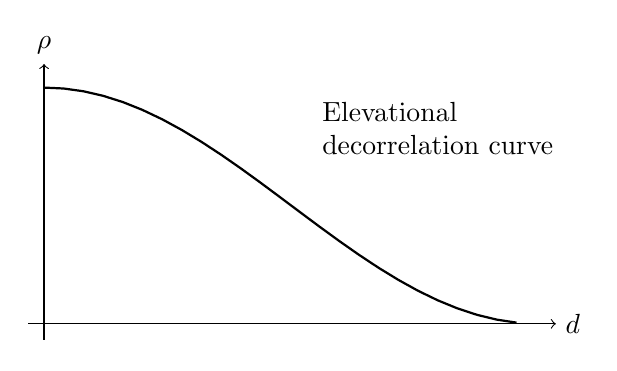
\begin{tikzpicture}[domain=0:6]
		\draw[color=black, ->] (-0.2,0) -- (6.5,0) node[right] {$d$};
		\draw[color=black, ->] (0,-0.2) -- (0,3.3) node[above] {$\rho$};
		
		% TikZ does not have a sinc function build-in, so fake it with cos
		\draw[color=black, thick] plot (\x, {1.5 * (cos(0.5 * \x r) + 1)}) node[above, xshift=-1cm, yshift=2cm, align=left] {Elevational \\ decorrelation curve};
	\end{tikzpicture}
	\caption{
		\textbf{Elevational decorrelation curve} describing the distance between two adjacent ultrasound frames given their correlation $\rho$ \cite{Housden07,Chen97,Afsham14}.
	}
	\label{fig:uscompounding:correlation-curve}
\end{figure}

Technically, the elevational decorrelation curve describing the distance $d$ of two frames given a correlation $\rho$ is of non-linear form (cf. Fig. \ref{fig:uscompounding:correlation-curve}) and needs to be carefully calibrated to the used ultrasound transducer \cite{Housden07,Chen97,Afsham14}.
However, since we assume to have tracking information available, we do not need to solely rely on speckle decorrelation and can approximate the elevational speckle curve by a linear function, which allows for a generic formulation.
For two tracked ultrasound frames $i, j$ with centroids $c_i, c_j$, we consider their correlation to be zero if their Euclidean distance exceeds a threshold $d_\text{max}$, while their correlation should be maximal if $c_i = c_j$.
Therefore, we define
\begin{equation}
	\label{eq:uscompounding:distance-term}
	D(i, j) := \max \left( \frac{d_\text{max} - \|c_i - c_j\|}{d_\text{max}} , \ 0 \right),
\end{equation}
which normalizes the correlation to the interval of $[0, 1]$.
A value of 1mm for $d_\text{max}$ showed excellent results for all our experiments.
While yielding comparable results for standard cases, this distance-based correlation term is not only simpler than the original Gaussian window formulation in \cite{Schultezub14}, but also a more robust generalization since it does also allow for non-homogeneous frame sampling rates.

We model the orientation-based correlation between two ultrasound frames by the cosine distance of their normals.
Thus, for two tracked ultrasound frames $i, j$ with normals $n_i, n_j$, we define the orientation-based correlation term as
\begin{equation}
	\label{eq:uscompounding:cosine-similarity}
	O(i, j) := \max \left( 1 - \frac{2}{\pi} \cdot \text{acos} \left( \frac{n_i \cdot n_j}{\|n_i\| \|n_j\|} \right) , \ 0 \right),
\end{equation}
which is a simple extension of the Euclidean dot product formula, normalized to yield results in the interval of $[0, 1]$.
In both terms, the maximum function avoids negative correlations.


\section{Orientation-driven Inter-frame Registration of Ultrasound Sweeps}
\label{sec:uscompounding:pressure-comp}

\begin{figure}[ht]
	\centering
	\subfloat[]{
		\label{fig:uscompounding:phantom_pressure_original}
		\includegraphics[height=5.5cm]{figures/uscompounding/phantom_pressure_original.jpg}
	}
	\subfloat[]{
		\label{fig:uscompounding:phantom_pressure_compensated}
		\includegraphics[height=5.5cm]{figures/uscompounding/phantom_pressure_compensated.jpg}
	}
	\subfloat[]{
		\label{fig:uscompounding:phantom_no_pressure}
		\includegraphics[height=5.5cm]{figures/uscompounding/phantom_no_pressure.jpg}
	}
	\caption{Reconstruction of an \textbf{abdominal phantom scan with probe pressure changes}: (a) MPR through the compounded volume without applying our pressure compensation technique; (b) the same MPR through the compounded volume with pressure compensation applied. For comparison, (c) shows the same target acquired using constant probe pressure.}
	\label{fig:uscompounding:comparison-pressure}
\end{figure}

To correct for errors and inaccuracies in the tracking data (e.g. due to jitter, inaccurate calibration or patient movement), we use the above framework for performing an intensity-based inter-frame registration, similar to Treece et al. \cite{Treece02}.
% Similar to Treece et al. \cite{Treece02}, we perform an intensity-based registration between adjacent ultrasound frames.
Since the image changes are minimal for adjacent ultrasound frames in a sweep, a simple and thus real-time capable pixel-wise uphill search evaluating the SSD is sufficient for registering each ultrasound frame to its surrounding frames in terms of in-plane translation and in-plane rotation.
To effectively compensate for registration drift, we regularize  by registering each ultrasound frame to a window of $N$ surrounding frames.
Thus, for a given reference patch $P$ and equally sized moving patch $P'$ the windowed SSD (wSSD) is given by
\begin{equation}
	\label{eq:uscompounding:wssd}
	\text{wSSD}_{P, P', N} (i) = \sum_{
		\substack{(p, p') \\ \in P \times P'}
	} \sum_{n = -N}^{N}  C(i, i+n) \cdot \big( I_i(p) - I_{i+n}(p') \big)^2,
\end{equation}
where $i$ is the index of the reference frame and $I_i(p)$ denotes the image intensity of ultrasound frame $i$ at the position $p$.


The central part in Eq. \ref{eq:uscompounding:wssd} is the correlation term $C(i, j)$, which describes the correlation between frames $i$ and $j$ and weights the surrounding frames' contribution to the similarity measure.
As motivated in the previous section, the correlation between the two frames depends on both their proximity and their orientation to each other.
Therefore, we define the $C(i, j)$ as
\begin{equation}
	\label{eq:uscompounding:correlation-term}
	C(i,j) := D(i,j) \cdot O(i,j).
\end{equation}

To compensate for probe pressure artifacts, we apply the above inter-frame registration technique not only to a single patch, but to a grid of independent patches of $10\text{mm} \times 10\text{mm}$ size.
We make the simplified assumption that for our applications a deformation model is sufficient, which expects the deformation to be only in transducer direction. 
Therefore, we allow in-plane translations of the individual patches.
After computing the transformation for each patch as above, we regularize the deformation field using a Gaussian  convolution, which corresponds to one iteration of a fluid-type demons registration \cite{Nielsen96,Thirion98,Zikic11} on the abovementioned grid.
We compute the coarse inverse deformation field using fixed-point iteration \cite{Chen08}, which is eventually extended to pixel level using bilinear filtering during the compounding process.
A exemplary result is displayed in Fig. \ref{fig:uscompounding:comparison-pressure}.



\section{An Information-fusion Approach to Ultrasound Compounding}
\label{sec:uscompounding:clustering}

Compounding ultrasound frames acquired from different viewpoints is non-trivial since ultrasound may show different intensities for the same anatomy if it is scanned from a different angle or at a different time.
This is due to the complex ultrasound image formation being dependent on many different factors such as view angle, probe pressure, patient position and breathing cycle.
Thus, tortuous acquisition sweeps are particularly challenging to reconstruct since their frames overlap.
Traditional compounding schemes based on averaging or distance-based weighting fail in correctly reconstructing such regions as illustrated in Fig. \ref{fig:uscompounding:different_angles_artifacts}.
Since closer pixels are preferred over pixels being farther away, the compounded voxel intensity mainly depends on the ultrasound frame of highest proximity.
If we now consider a neighbor voxel, the closest frame may have a completely different orientation and thus show different information (due to the view dependency of ultrasound).
The resulting reconstructions exibit a low image quality with significant discontinuities in the anatomy.
Furthermore, unwanted stripe or pixel artifacts may arise as depicted in Fig. \ref{fig:uscompounding:stripe-artifacts}. 

Besides promoting artifacts and inhomogenities, distance-based weighting can also lead to incorrect reconstruction results since the distance of the frame to the voxel has no correlation with the amount of information present in this pixel (i.e. level of uncertainty/noise).
For instance, it may ignore a pixel being farther away but having low uncertainty and instead prefer a high uncertainty pixel (i.e. noise) because it is closer to the voxel.

These two issues are the main motivation for our proposed orientation-driven ultrasound compounding technique.
It tackles them by partitioning the ultrasound sweep into clusters of similar alignment and then using additional uncertainty information in a two-step fusion approach.
We assume that for each ultrasound pixel with intensity $I_i$, we also have an uncertainty value $u_i$ that we will use for weighting the image intensities during compounding.
While our method considers the generation of uncertainty information as black box and is thus independent from it, we use for our implementation the Confidence Maps as proposed by Karamalis et al. \cite{Karamalis12}.
Even though they model ultrasound physics only to a limited amount, their Confidence Maps can be interpreted as uncertainty information. 

\begin{figure}[t]
	\centering
	\resizebox{0.75\linewidth}{!}{
		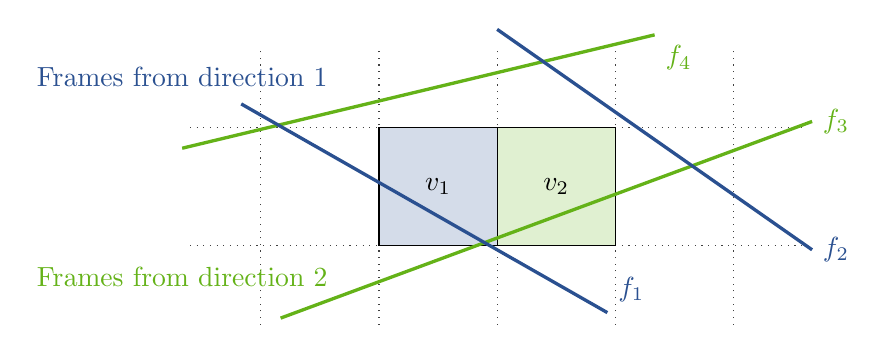
\begin{tikzpicture}[
	vertexlabel/.style={outer sep=6pt, fill=white},
	endpoint/.style={color=tumblue!75},
	midpoint/.style={color=tumblue!40},
	cluster1/.style={dagreen, very thick},
	cluster2/.style={tumblue, very thick}
	]
		\definecolor{dagreen}{RGB}{100, 178, 24}	
		\definecolor{tumblue}{RGB}{42, 80, 144}	
% 	\coordinate [label={[vertexlabel]below:{$v_0 = (x_0, y_0, z_0)$}}] (v0) at (-1.65, -2.2);
% 	\coordinate [label={[vertexlabel]above left:{$v_1 = (x_1, y_1, z_1)$}}]  (v1) at (-2.60,  0.9);
% 	\coordinate [label={[vertexlabel]below right:{$v_2 = (x_2, y_2, z_2)$}}] (v2) at ( 2.60, -0.9);
% 	\coordinate [label={[vertexlabel]above:{$v_3 = (x_3, y_3, z_3)$}}] (v3) at ( 1.65,  2.2);

	% grid
	\draw[step=1.5cm, darkgray,dotted, thin] (-3.9, -1.0) grid (3.9, 2.5);
		
	% voxel 1
	\filldraw [fill=tumblue!20] (-1.5, 0) rectangle (0, 1.5);
	\node at (-0.75, 0.75) {$v_1$};
	
	% voxel 2
	\filldraw [fill=dagreen!20] (0, 0) rectangle (1.5, 1.5);
	\node at (0.75, 0.75) {$v_2$};
	
	% Frames cluster 1
	\node [cluster1] at (-4, -0.4) {Frames from direction 2};
	\draw [cluster1, domain=-2.75:4] plot (\x, {0.37*\x + 0.1}) node[right] {$f_3$};
	\draw [cluster1, domain=-4:2.0] plot (\x, {0.24*\x + 2.2}) node[below right] {$f_4$};
	
	% Frames cluster 2
	\node [cluster2] at (-4, 2.15) {Frames from direction 1};
	\draw [cluster2, domain=-3.25:1.4] plot (\x, {-0.57*\x - 0.05}) node[above right] {$f_1$};
	\draw [cluster2, domain=-0.0:4.00] plot (\x, {-0.7*\x + 2.75}) node[right] {$f_2$};
\end{tikzpicture}

	}
	\caption{
		Illustration of \textbf{artifacts occurring in distance-weighted compounded regions} where multiple ultrasound frames from different directions intersect.
		With traditional methods, voxel $v_1$ is mainly based on the information of frame $f_1$ while its neigbour voxel $v_2$ is mainly based on the information in frame $f_3$.
			However, their intensities at this spatial location may significantly differ since the frames travel through different acoustic windows.
	}
	\label{fig:uscompounding:different_angles_artifacts}
\end{figure}

\begin{figure}[ht]
	\centering
	\subfloat[]{
		\includegraphics[width=0.95\textwidth]{figures/uscompounding/cluster-bs.jpg}
		\label{fig:uscompounding:stripe-artifacts}
	}
	\\
	\subfloat[]{
		\includegraphics[width=0.95\textwidth]{figures/uscompounding/cluster-od.jpg}
	}
	\caption{
		Effect of the \textbf{orientation-driven clustering} of ultrasound frames:
		Both images show reconstructions of a tortuous sweep of upper arm ultrasound.
		(a) Traditional techniques with distance-only weighting show severe stripe artifacts (yellow arrows) in regions of overlapping frames.
		(b) Partitioning the sweep into clusters of homogeneous orientation and fusing the clusters based on uncertainty suppreses these artifacts almost entirely.
		Please mind that both volumes were compounded \emph{without} applying our pressure compensation technique to highlight the beneficial effect of the orientation-driven clustering.
	}
	\label{fig:uscompounding:comparison-clustering}
\end{figure}

\subsection{Clustering of Ultrasound Sweeps by Direction}
As a first step, we perform a hierarchical clustering to identify tortuous sweep trajectories and regions of overlapping ultrasound frames.
This partitions the ultrasound sweep trajectory into parts where the frames have homogeneous orientation without requiring us to predefine the number of clusters.
We apply an average group linkage algorithm on the previously defined orientation term $O(i, j)$ (cf. Eq. \ref{eq:uscompounding:cosine-similarity}).
This yields a set $C$ of sub-sweeps meeting the usual restriction of being contiguous and uniformly oriented.

\subsection{Compounding of each Cluster}
\label{sec:uscompounding:compounding-of-each-cluster}
A backward warping algorithm then compounds each cluster $c \in C$ into a 3D volume $I_c$ applying our pressure compensation method as discussed in Section \ref{sec:uscompounding:pressure-comp}.
Since the ultrasound frames of each cluster are guaranteed to have the same orientation and are thus travelling through the same acoustic window, we can safely assume the uncertainty distribution to be homogeneous within nearby frames.
We compute the intensity for voxel $x$ as
\begin{equation}
	I_c(x)		=		\frac{\sum_{i\in S} I_i \cdot d_i^{-\mu}}{\sum_{i \in S} d_i^{-\mu}},
\end{equation}
where $S$ is the set of frame pixels close to the compounded voxel $x$, $d_i$ the Euclidean distance of pixel $i$ to the compounded voxel, and $\mu>1$ a smoothness parameter ensuring that $I_c(x)$ approximates the original data for $d_i \rightarrow 0$ \cite{Shepard68}.
Wein et al. showed that this inverse distance weighting scheme yields excellent results in terms of image quality \cite{Wein06}.
We use the same weighting to propagate the uncertainty to a separate 3D volume $U_c$:
\begin{equation}
	U_c(x)		=		\frac{\sum_{i\in S} u_i \cdot d_i^{-\mu}}{\sum_{i \in S} d_i^{-\mu}}.
\end{equation}

Thus, for each cluster $c \in C$ we end up with a compounded ultrasound intensity volume $I_c$ and a compounded uncertainty volume $U_c$.


\subsection{Uncertainty-based Fusion of the Compounded Clusters}
% Since ultrasound image formation is a highly non-linear process and the pixel-based uncertainty values $u_i$ are relative to the image content and thus not necessarily comparable between different frames, we perform the uncertainty-based fusion in a second step to avoid artifacts such as the ones depicted in Fig. \ref{fig:uscompounding:stripe-artifacts}.
In a final step, our method fuses the clusters together into the final 3D volume based on the propagated uncertainty values.
We want the individual clusters $c \in C$ to contribute in an additive manner weighted by the propagated voxel uncertainties.
Therefore, we compute the final intensity $I$ at voxel $x$ by
\begin{equation}
	\label{eq:uscompounding:fusion}
	I(x)		=		\frac{\sum_{c\in C} (1 - U_c(x)) I_c(x)}{\sum_{c \in C} 1 - U_c(x)}.
\end{equation}

Since we are acquiring a continuous sweep of ultrasound frames and apply a regularized inter-frame registration with active pressure compensation, we can safely assume that the individual clusters are well aligned.
Hence, an additional 3D-3D registration is not needed.


\section{Incremental Compounding System}
For interventional usage, one does not only require short processing times, but also wants to support an interactive update of the compounded volume during the acquisition to allow for an additional refinement of selected regions.
Therefore, we introduce \emph{incremental ultrasound compounding} as a real-time capable extension of our orientation-driven compounding technique.

\subsection{Incremental Compounding Pipeline}
As illustrated in Fig. \ref{fig:uscompounding:schematic-diagram}, our system receives a constant stream of incoming ultrasound frames.
The regularized inter-frame registration (cf. Section \ref{sec:uscompounding:pressure-comp}) needs only a limited number of frames lookahead (i.e. size of the regularization window) and can hence be performed on-line requiring only a small number of frames to be buffered.
We extend the orientation-driven clustering approach (cf. Section \ref{sec:uscompounding:clustering}) to a partitioning into batches of ultrasound frames.
In addition to starting new clusters when the correlation term exceeds the threshold, we also start new batches in a regular time interval (e.g. every second) to keep their size small.


Instead of reconstructing a separate volume for each batch, we use a single volume as accumulation buffer and adapt the above technique to an in-place algorithm.
The reconstructed voxels of each cluster can be incrementally added to an accumulation buffer by rewriting Eq. \ref{eq:uscompounding:fusion} to a recurrence scheme. 
Given the accumulated compounded intensity $I_{i-1}$ and accumulated compounded uncertainty $U_{i-1}$ of the previous runs, and $I_c, U_c$ of the current run, we define the new intensity $I_i$ and uncertainty $U_i$ as
\begin{equation}
	\label{eq:uscompounding:incremental-fusion}
	\begin{split}
		I_i		&=		\frac{U_{i-1} I_{i-1}   +   (1 - U_c) I_c}{U_{i-1}   +  (1 - U_c)}, \\
		U_i		&=		U_{i-1}   +  (1 - U_c).
	\end{split}
\end{equation}
This transforms our technique into an on-line algorithm, significantly lowering the computational complexity and memory footprint and furthermore allowing for an interactive update of the visualization after each batch.

Apart from a slightly worse (but in our case neglectable) numerical stability, Eq. \ref{eq:uscompounding:fusion} and Eq. \ref{eq:uscompounding:incremental-fusion} yield the same reconstruction result.
It should be noted that, with the incremental clustering, frames of the same orientation may end up in different clusters compared to the conventional formulation when they are separated by frames of different orientation.
While technically this may alter the final result, we did not observe any qualitative differences in our experiments.


\begin{figure}[ht]
	\centering
	\subfloat[No pressure compensation applied.]{
		\includegraphics[width=0.31\textwidth]{figures/uscompounding/registration0x0.jpg}
	}
	\;
	\subfloat[Inter-frame registration with $3 \times 4$ patches yielding a patch size of $10\text{mm} \times 10.5\text{mm}$.]{
		\includegraphics[width=0.31\textwidth]{figures/uscompounding/registration3x3.jpg}
	}
	\;
	\subfloat[Inter-frame registration with $4 \times 20$ patches yielding a patch size of $7.5\text{mm} \times 2.1\text{mm}$.]{
		\includegraphics[width=0.31\textwidth]{figures/uscompounding/registration5x16.jpg}
	}
	\caption{
		Multi-planar reconstructions of in-vivo acquisitions of the Infraspinatus muscle showing the \textbf{effectiveness of the pressure compensation}.
		Though the sweep was acquired by a professional sonographer trying to maintain constant probe pressure, the result of a traditional compounding technique (a) has an unsteady appearance and shows discontinuities throughout the different muscle layers.
		Applying our orientation-driven inter-frame registration and pressure compensation even on low resolution grid with $10\text{mm} \times 10.5\text{mm}$ patch size (b) yields a significant increase in image quality.
		Further increasing the resolution of the deformation field to $7.5\text{mm} \times 2.1\text{mm}$ patch size (c) yields only slight improvements.
	}
	\label{fig:uscompounding:comparison-registration}
\end{figure}

\subsection{Real-time Implementation}
The most time-consuming part of our reconstruction pipeline is the incremental compounding of each batch of ultrasound frames into the target volume.
To yield high quality results, we employ a backward compounding technique where each voxel of the target volume is compared to each ultrasound frame to find contributing pixels (cf. Section \ref{sec:uscompounding:compounding-of-each-cluster}).
This process can be parallelized heavily on voxel level.
To exploit the new features of recent graphics hardware, we implemented the entire incremental compounding process on the GPU using OpenGL 4.3.
To this end, we store the tracking information as well as other required data in Shader Storage Buffer Objects \cite{OpenGL43,SSBO} and the image data of the ultrasound frames in 2D texture arrays to support hardware-accelerated interpolation during sampling.
This allows us to yield highly interactive frame rates for the compounding process.
This is further accelerated by exploiting that we do not need to traverse the voxels of the entire target volume but can restrict the reconstruction volume of each pass to the bounding box of the corresponding batch of ultrasound frames.
Our information fusion approach exploiting uncertainty information ensures that the additional partitioning of the ultrasound sweep into batches does not impair the reconstruction quality.


\section{Results and Evaluation}
To evaluate our methods, we used an Acuson S2000\texttrademark~ultrasound machine equipped with an Acuson 9L4 linear transducer and Ascension trakSTAR\texttrademark 2 electromagnetic tracking hardware.
The system was calibrated using the method described in \cite{Wein08}, yielding an experimental calibration error of less than 2mm and 4 degrees.
We acquired both phantom and in-vivo data of different anatomies where the in-vivo sweeps were acquired by a professional sonographer.
All baseline results for comparison within this section were computed using our own implementation of a state-of-the-art backward compounding technique with inverse distance weighting as proposed by Wein et al. \cite{Wein06}.


\subsection{Parameter Evaluation}
To evaluate the effectiveness of our orientation-driven inter-frame registration and pressure compensation, and its dependency on parameters, we applied our technique to different ultrasound sweeps of both phantom and in-vivo data.
Figures \ref{fig:uscompounding:comparison-pressure} and \ref{fig:uscompounding:comparison-registration} show representative results.

All experiments show a significant improvement in terms of image appearance and continuity of anatomy features when applying inter-frame registration, even with only minimal pressure changes present in the input data.
In particular, the in-vivo scans show good results already with low resolution deformation fields, such as $3 \times 4$ patches for the Infraspinatus data set resulting in a patch size of roughly $10\text{mm} \times 10\text{mm}$.
Increasing the deformation field resolution by decreasing the patch size yields only marginal improvements while increasing the computational burden (cf Fig. \ref{fig:uscompounding:comparison-registration}).
Hence, in our implementation, we use a target patch size of $10\text{mm} \times 10\text{mm}$ as default setting.



\subsection{Reconstruction Accuracy}
To validate the physically correct reconstruction of anatomy, we acquired ultrasound sweeps of an abdominal phantom including a tumor target of spherical shape as depicted in Fig. \ref{fig:uscompounding:comparison-pressure}.
Since the target is positioned relatively close to the surface, it can be scanned from different directions and is prone to deformation.
Therefore, this is a relevant scenario to evaluate our method.
We computed 50 MPRs of arbitrary orientation through the target and compared the maximum diameter with reference measurements acquired from CT. 
The reconstructed ultrasound volume yielded an average target diameter of $14.63 \pm 0.48$ mm  compared to $14.5 \pm 0.84$ mm in CT.
This proves an excellent physical accuracy of our reconstruction method.



\subsection{Reconstruction Quality}
The qualitative effects of our inter-frame registration and pressure compensation technique can be observed in Fig. \ref{fig:uscompounding:comparison-pressure} and \ref{fig:uscompounding:comparison-registration} showing the reconstructions of different ultrasound sweeps. 
The originally round target of the abdominal phantom (Fig. \ref{fig:uscompounding:phantom_no_pressure}) is severely deformed through probe pressure changes (Fig. \ref{fig:uscompounding:phantom_pressure_original}).
Our pressure compensation technique is capable of mostly restoring the original anatomy (Fig. \ref{fig:uscompounding:phantom_pressure_compensated}).
While the original shape is not perfectly restored, there is a clear improvement visible.
Also Fig. \ref{fig:uscompounding:comparison-registration} shows significant improvements in terms of continuity of anatomy when enabling our pressure compensation.
Compared to \cite{Treece02}, there is still room for improvement. 
However, we want to emphasize that the implemented pressure compensation is of only complementary nature and the focus of this work is die orientation-driven clustering and compounding technique.

Fig. \ref{fig:uscompounding:comparison-clustering} demonstrates the effect of our clustering technique when reconstructing a twisted ultrasound sweep of a human arm exhibiting out-of-plane rotations of up to 35 degrees.
Due to overlapping frames, the standard compounding in (a) shows artifacts at locations where the frames for neighboring voxels are acquired through different acoustic windows.
The reconstruction in (b) removes such artifacts by using our clustering technique to avoid overlapping frames in a single cluster. 
Additionally, it exploits uncertainty information when fusing the clusters so that unreliable intensities do not bias the final result.
Please note that, in order to highlight the effect of the clustering, these volumes were reconstructed without  pressure compensation and thus show discontinuities in the anatomy.

\begin{figure}[ht]
	\centering
	\includegraphics[width=0.75\textwidth]{figures/uscompounding/achilles_3d.jpg}
	
	\caption{
			\textbf{3D visualization of an achilles tendon} data set compounded with our technique.
			Due to the high curvature of the skin surface this is a challenging anatomy for sonography.
			Our clinical partners appreciate the high quality spatial reconstruction where possible lesions are easy to identify.
	}
	\label{fig:uscompounding:achilles-3d}
\end{figure}

To further illustrate a clinical application, Fig. \ref{fig:uscompounding:achilles-3d} shows a 3D visualization of an achilles tendon ultrasound volume acquired with our technique.
Due to the high curvature of the surrounding skin surface, this is a challenging anatomy for ultrasound compounding.
Our clinical partners highly appreciate the reconstruction quality where they can easily identify possible lesions in a spatial context.

To quantitatively evaluate the effectiveness of our orientation-driven compounding technique in terms of ensuring continuity of the anatomy and reducing artifacts in regions of overlapping ultrasound frames, we evaluate a local, scale-invariant entropy measure of the reconstructed sweeps.
For every voxel we computed the intensity difference to the neighboring voxels and computed the mean and standard deviation over the entire volume.
This measure penalizes high frequency intensity changes such as the mentioned stripe artifacts while preferring smooth and continuous reconstructions of the anatomy, which are desired for clinical and visualization purposes.
To avoid biasing the result, we considered only the inner part of the volume and masked the outer faces of the sweep, as they naturally have a high entropy.
The results as displayed in Table \ref{tbl:entropy} show that our technique is sucessful in reducing the amount of reconstruction artifacts.
While the entropy measures are not directly comparable between the data sets, all test data sets with a twisted probe trajectory show a significant drop in the mean difference and standard deviation.
As reference, the first line shows the measure for a data set with a strictly linear sweep trajectory.
Here, the drop in entropy turns out to be much lower.



\begin{table}[th]
	\centering
	\caption{		
			Quantification of the local entropy in compounded volumes in terms of mean intensity difference to neighboring voxels.
	}
	\label{tbl:entropy}
	\begin{tabu} to 0.95\linewidth {>{\bfseries\centering}m{55mm} C C}
		\toprule
		\                                & \bfseries Baseline \cite{Wein06} & \bfseries Our Technique \\
		\midrule
		In-vivo leg / linear sweep       & $2.65 \pm 2.42$                  & $2.49 \pm 2.39$         \\
		\midrule
		In-vivo arm	/ twisted sweep      & $4.59 \pm 8.42$                  & $2.44 \pm 4.62$         \\
		In-vivo leg	/ twisted sweep      & $3.58 \pm 5.82$                  & $2.34 \pm 4.19$         \\
		In-vivo carotid artery	/ twisted & $7.2 \pm 13.35$                  & $3.17 \pm 8.58$         \\
		In-vivo infraspinatus	/ twisted  & $4.17 \pm 7.21$                  & $2.99 \pm 6.17$         \\
		\bottomrule
	\end{tabu}
\end{table}

\begin{figure}[ht]
	\centering
	\subfloat[Baseline]{
		\label{fig:uscompounding:msd_baseline}
		\includegraphics[width=0.48\textwidth]{figures/uscompounding/difference2_baseline.png}
	}
	\subfloat[Our Technique]{
		\label{fig:uscompounding:msd_ours}
		\includegraphics[width=0.48\textwidth]{figures/uscompounding/difference2_ours.png}
	}
	\caption{
		\textbf{Illustration of our evaluation method}: First two images show the MPRs for each perpendicular sweep, the third one shows the color-coded absolute difference of their intensities after 3D-3D rigid registration.
		(a) traditional backward-compounding \cite{Wein06} fails to align the different structures; 
		(b) our technique yields alignment of all structures.
		The quantitative results are shown in Table \ref{tbl:registration-results}.
	}
	\label{fig:uscompounding:comparison-msd}
\end{figure}

For further quantitative evaluation we acquired pairs of overlapping sweeps with perpendicular main trajectory.
After compounding the sweeps into separate 3D volumes using our methods, we applied a 3D-3D rigid registration using the tracking data as initialization.
Expecting our techniques to yield better matching volumes, we compared the differences of the two volumes in the overlapping region.
With the average of the two volumes as expected result for a correct reconstruction, we quantify their difference in Normalized Cross-Correlation (NCC) and log-scale Signal to Noise Ratio (SNR\textsubscript{dB}), for which define the signal as average of the volumes and the noise as RMS of the differences (Table \ref{tbl:registration-results}).

\begin{table}[th]
	\centering
	\caption{NCC and log-scale SNR in the overlapping region after registering the two compounded volumes of two sweeps with perpendicular trajectories of the same anatomy.}
	\label{tbl:registration-results}
	\begin{tabu} to 0.95\linewidth {>{\bfseries\centering}m{55mm} CC CC}
		\toprule
		\quad                          & \multicolumn{2}{c}{\bfseries Baseline \cite{Wein06}} & \multicolumn{2}{c}{\bfseries Our technique} \\
		\quad                          & NCC    &        SNR\textsubscript{dB}        & NCC    &  SNR\textsubscript{dB}   \\
		\midrule
		Phantom / constant pressure    & $0.90$ &               $19.39$               & $0.94$ &         $23.16$          \\
		Phantom / pressure changes     & $0.81$ &               $13.02$               & $0.94$ &         $22.47$          \\
		\midrule
		In-vivo leg / constant changes & $0.72$ &               $ 9.21$               & $0.76$ &         $11.69$          \\
		In-vivo leg / pressure changes & $0.67$ &               $ 8.53$               & $0.75$ &         $11.03$          \\
		\bottomrule
	\end{tabu}
\end{table}

The sweeps with pressure changes show a significant improvement in terms of increase in both NCC and SNR\textsubscript{dB} when our technique is applied.
Furthermore, when comparing constant pressure with pressure changes, our technique shows significantly less drop of the measures.
The slight improvements for the sweeps acquired with constant pressure are mainly due to the inter-frame registration correcting for the tracking error.
Since the sweeps are acquired with perpendicular trajectories and the volumes therefore show different interpretations of the underlying data, no algorithm yields a perfect match.
Furthermore, the in-vivo sweeps are expected to have lower similarity since they show by far less homogeneous anatomy.
Figure \ref{fig:uscompounding:comparison-msd} shows the difference images for the second phantom sweep.




\subsection{System Performance}
For the evaluation of the system performance, we ran our implementation on a workstation with an Intel Core\texttrademark~ i7-4770 CPU and a nVidia GeForce\texttrademark~ GTX 670 GPU.
We loaded recordings of different ultrasound acquisitions, streamed them into our incremental compounding pipeline and measured the time required for computing the final reconstructed volume at different resolutions. 

\begin{table}[th]
	\centering
	\caption{
		System performance of our incremental compounding technique at different target volume resolutions.
		The timings measure the compounding only (no generation of uncertainty information or visualization).
	}
	\label{tbl:performance}
	\begin{tabu} to 0.95\linewidth {m{2mm}m{32mm} C C C}
		\toprule
		& \bfseries Voxel Size		& \bfseries Volume Size										& \bfseries Time					& \bfseries Speed \\
		\midrule
		\multicolumn{2}{l}{\bfseries In-vivo arm} & & & \\ %\multicolumn{3}{c}{\addd{500 frames}} \\
		& $0.5$ mm			& $160 \times 119 \times 157$		& 728 ms 				& 687 fps \\
		& $0.25$ mm			& $320 \times 237 \times 313$		& 1551 ms				& 322 fps \\
		& $0.1$ mm			& $800 \times 591 \times 781$		& 13499 ms			& 37 fps \\
		\midrule
		\multicolumn{2}{l}{\bfseries In-vivo leg} & & & \\ %\multicolumn{3}{c}{\addd{241 frames}} \\
		& $0.5$ mm			& $187 \times 138 \times 101$		& 389 ms				& 620 fps \\
		& $0.25$ mm			& $373 \times 276 \times 214$		& 906 ms				& 266 fps \\
		& $0.1$ mm			& $931 \times 689 \times 533$		& 8433 ms			  & 29 fps \\
		\midrule
		\multicolumn{2}{l}{\bfseries In-vivo carotid artery} & & & \\ %\multicolumn{3}{c}{\addd{488frames}} \\
		& $0.5$ mm			& $90 \times 62 \times 97$			& 657 ms 				& 743 fps \\
		& $0.25$ mm			& $179 \times 124 \times 194$		& 735 ms				& 664 fps \\
		& $0.1$ mm			& $447 \times 308 \times 485$		& 2569 ms				& 189 fps \\
		\midrule
		\multicolumn{2}{l}{\bfseries In-vivo infraspinatus} & & & \\ %\multicolumn{3}{c}{\addd{370 frames}} \\
		& $0.5$ mm			& $114 \times 104 \times 178$		& 609 ms 				& 608 fps \\
		& $0.25$ mm			& $228 \times 207 \times 355$		& 1135 ms				& 326 fps \\
		& $0.1$ mm			& $570 \times 517 \times 887$		& 6761 ms				& 55 fps \\
		\bottomrule
	\end{tabu}
\end{table}

Table \ref{tbl:performance} shows the timings for four exemplary data sets.
The performance mainly depends on the number of frame pixels contributing to a single voxel (i.e. relationship between pixel size, voxel size and frame sampling rate) as well as the number of identified clusters (i.e. tortuosity of the sweep).
The results show that for a clinically adequate resolution of $0.25$ mm voxel size, our system has enough bandwidth to reconstruct ultrasound sweeps of very high framerate.
Even high-quality reconstructions of $0.1$ mm voxel size can be compounded at interactive frame rates.


\section{Conclusion}
In this work, we presented a novel orientation-driven approach featuring an incremental compounding scheme. 
We developed our methods with the aim to free clinicians from the restrictive scanning protocols of many of today's state of the art methods, which require the acquisition of linear probe trajectories and constant probe pressure.
Our target application within this work was MSK ultrasound, where typical sweeps exhibit pressure changes, back- and forth and twisting motion.
Therefore, we introduced a framework of two correlation terms to capture that the correlation of two frames in an ultrasound sweep depends on their proximity and orientation to each other.
This framework is used to perform a complementary pressure compensation as well as a clustering of ultrasound frames by orientation to remove different kinds of artifacts.
In the subsequent compounding process, we use an information fusion approach exploiting ultrasound Confidence Maps.
This allows for more accurate reconstructions in regions where we have information from different acoustic windows, since intensities from uncertain regions do not bias intensity information from reliable regions.
Finally, we presented an integrated system for incremental compounding that interactively fills the reconstructed volume while acquiring the sweep.
This provides the clinician with direct feedback on the ongoing acquisition and allows for an interactive refinement of target regions.


We evaluated the different aspects of our technique using both phantom and in-vivo data, which was acquired by a professional sonographer.
The results show that our methods accurately reconstruct the original anatomy and yield superior results than traditional backward compounding methods in terms of image quality, continuity of the anatomy and presence of artifacts.
Furthermore, the evaluation of our integrated incremental compounding system shows that the proposed system has enough bandwidth to reconstruct ultrasound sweeps with more than a hundred frames per second when using a clinically adequate target voxel size of 0.25mm.
Even with high resolution volumes of 0.1mm voxel size, we still can yield interactive frame rates to update the compounded volume during the acquisition.

Hence, we see our orientation-driven approach as an important step towards providing clinicians with more freedom regarding 3D freehand ultrasound scanning protocols so that they can focus on which images the acquire instead of on how they have to acquire them.
Current limitations of our work are mostly formed by the rather simple pressure compensation, which is not always capable of fully undoing all deformations.
Therefore, as further work, we would like to merge more sophisticated pressure compensation techniques, such as \cite{Treece02}, into our orientation-driven framework.

